\section{Sprints}


\subsection{Sprint 1}
Im ersten Sprint sicherten wir die Grundfnktionalität. 

Im ersten Sprint wollten wir sicher gehen, dass die Verbindung zwischen Sensor, Basisstation und App gewährleistet ist. Hierzu hatten wir folgende Kernpunkte:
\begin{itemize}
	\item App GUI Konzept 
	\item App GUI Grundgerüst
	\item Verbindung zwischen Basisstation und App
	\item Verbindung zwischen Smart Gadget und Basisstation
	\item Konzept Software-Layout Basisstation
	\item Benachrichtigung Push
	\item Klassen definieren die auf App und Basistation benutzt werden
	\item App Software Architektur Konzept
	\item Benachrichtigung
	\item Erstes Datenbankschema definieren
	\item Schnittstelle zwischen App und Basistation definieren
\end{itemize}

Wir konnten die Aufgaben wie in der Burndown chart ersichtlich fertigstellen.
\begin{figure}[htb] 
	\centerline{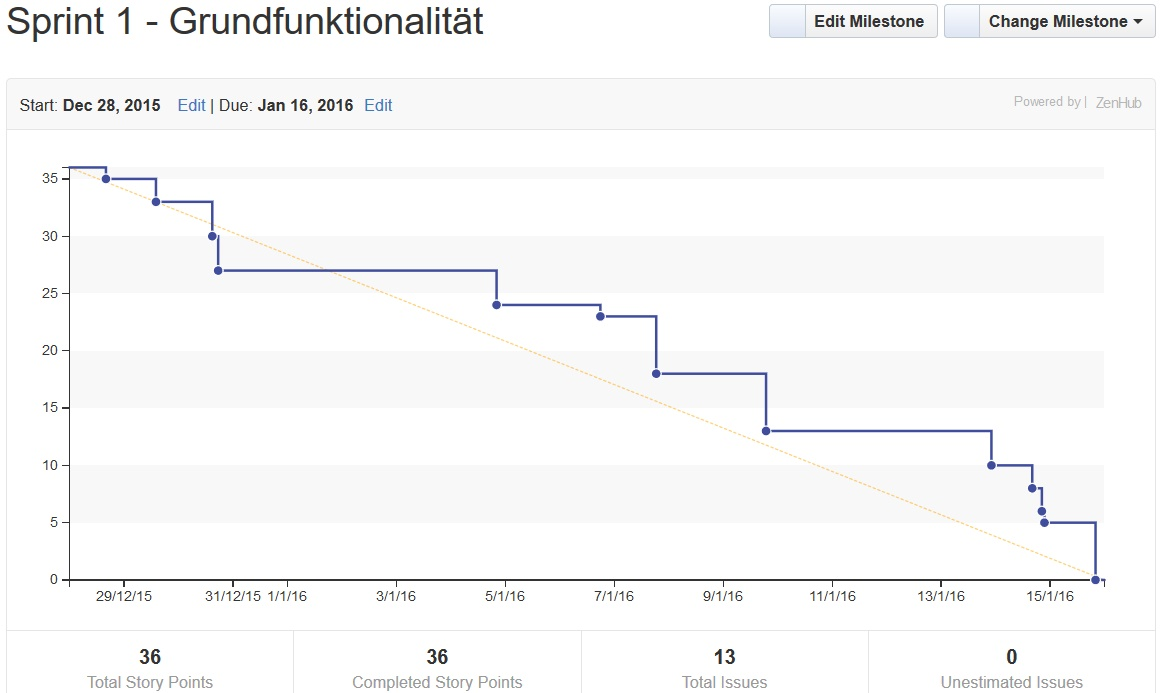
\includegraphics[width=0.7\textwidth]{burndown_sprint1.jpg}}
	\caption{Burndown chart des ersten (und längsten) Sprints}
	\label{screenshot_sprint_1_burndown}
\end{figure}
Innerhalb der App wurde die GUI fertig gestellt. (Abbildungen \ref{screenshot_sprint_1_laundry_status} und \ref{screenshot_sprint_1_navigation_drawer})
\begin{figure}[htb] 
	\centerline{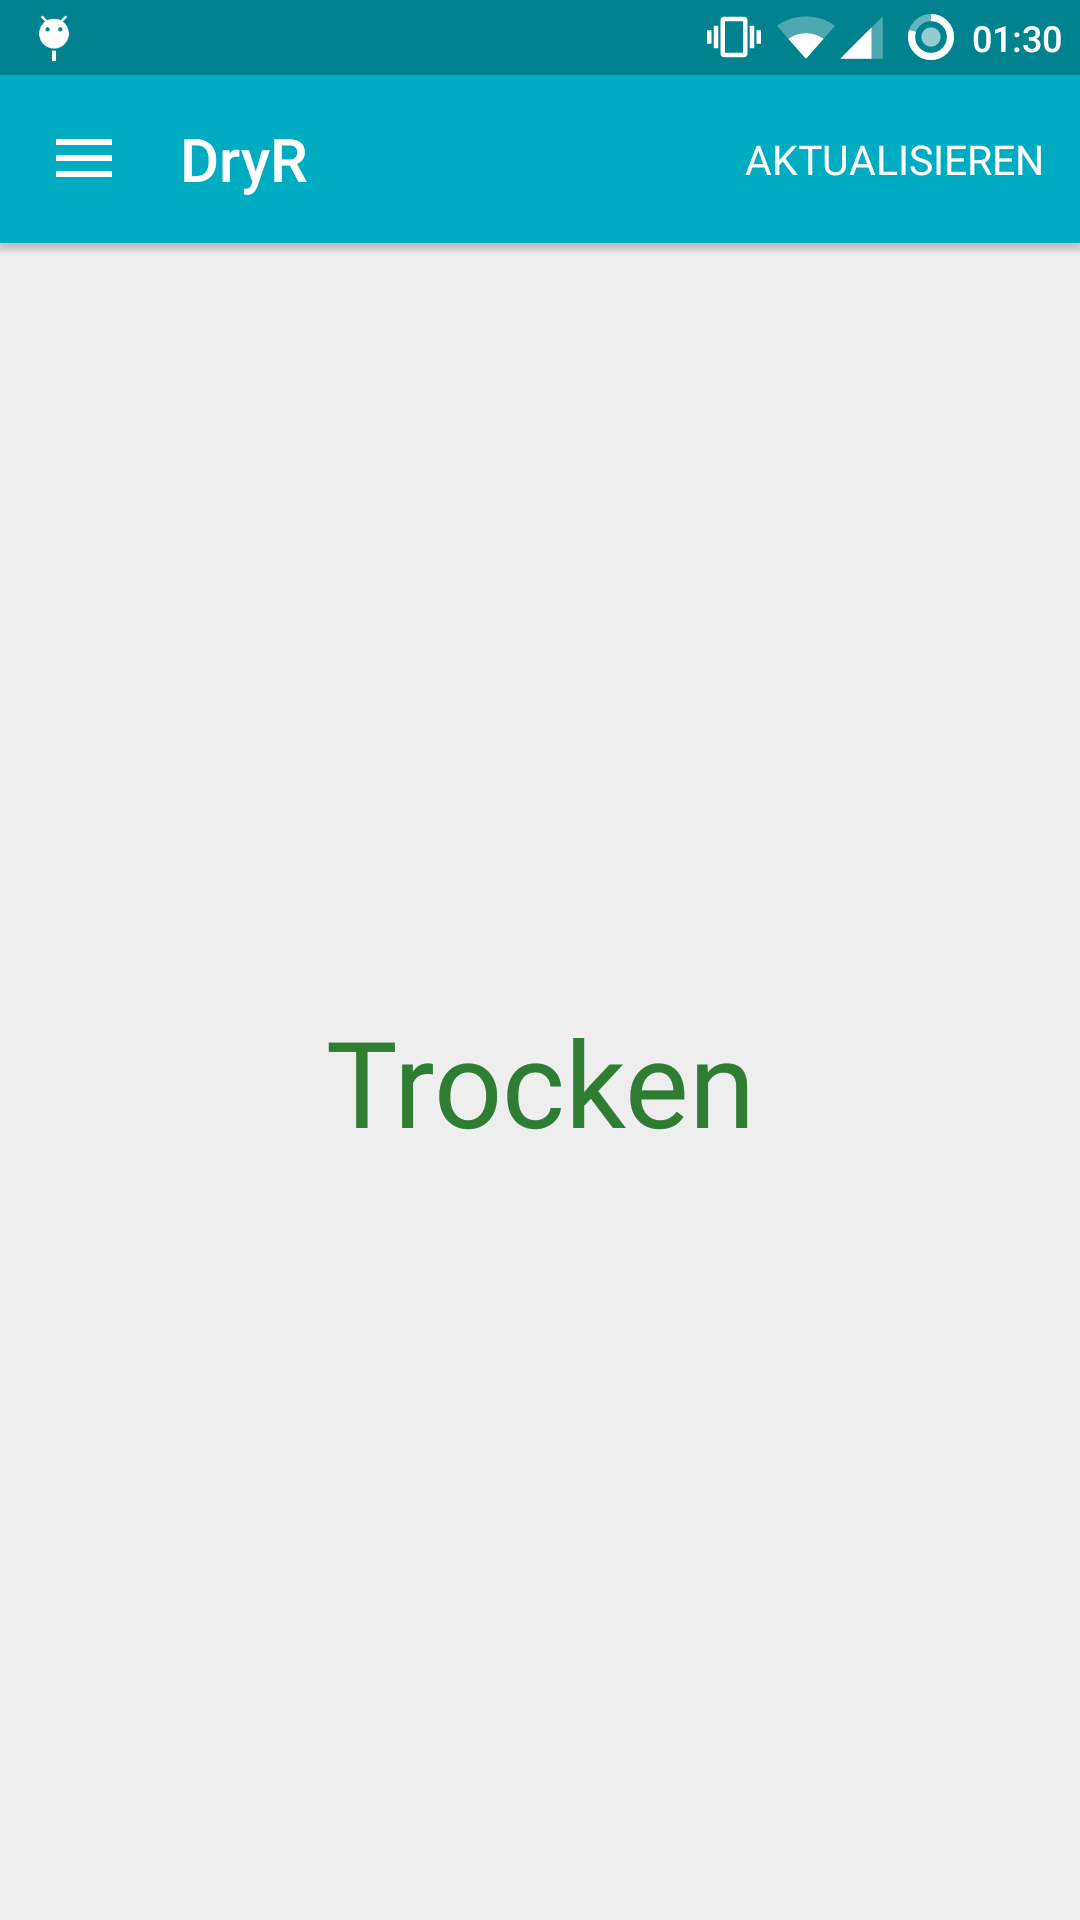
\includegraphics[width=0.5\textwidth]{laundry_status_dry.png}}
	\caption{Android App nach Sprint 1: Wäschestatusbildschirm}
	\label{screenshot_sprint_1_laundry_status}
\end{figure}
\begin{figure}[htb] 
	\centerline{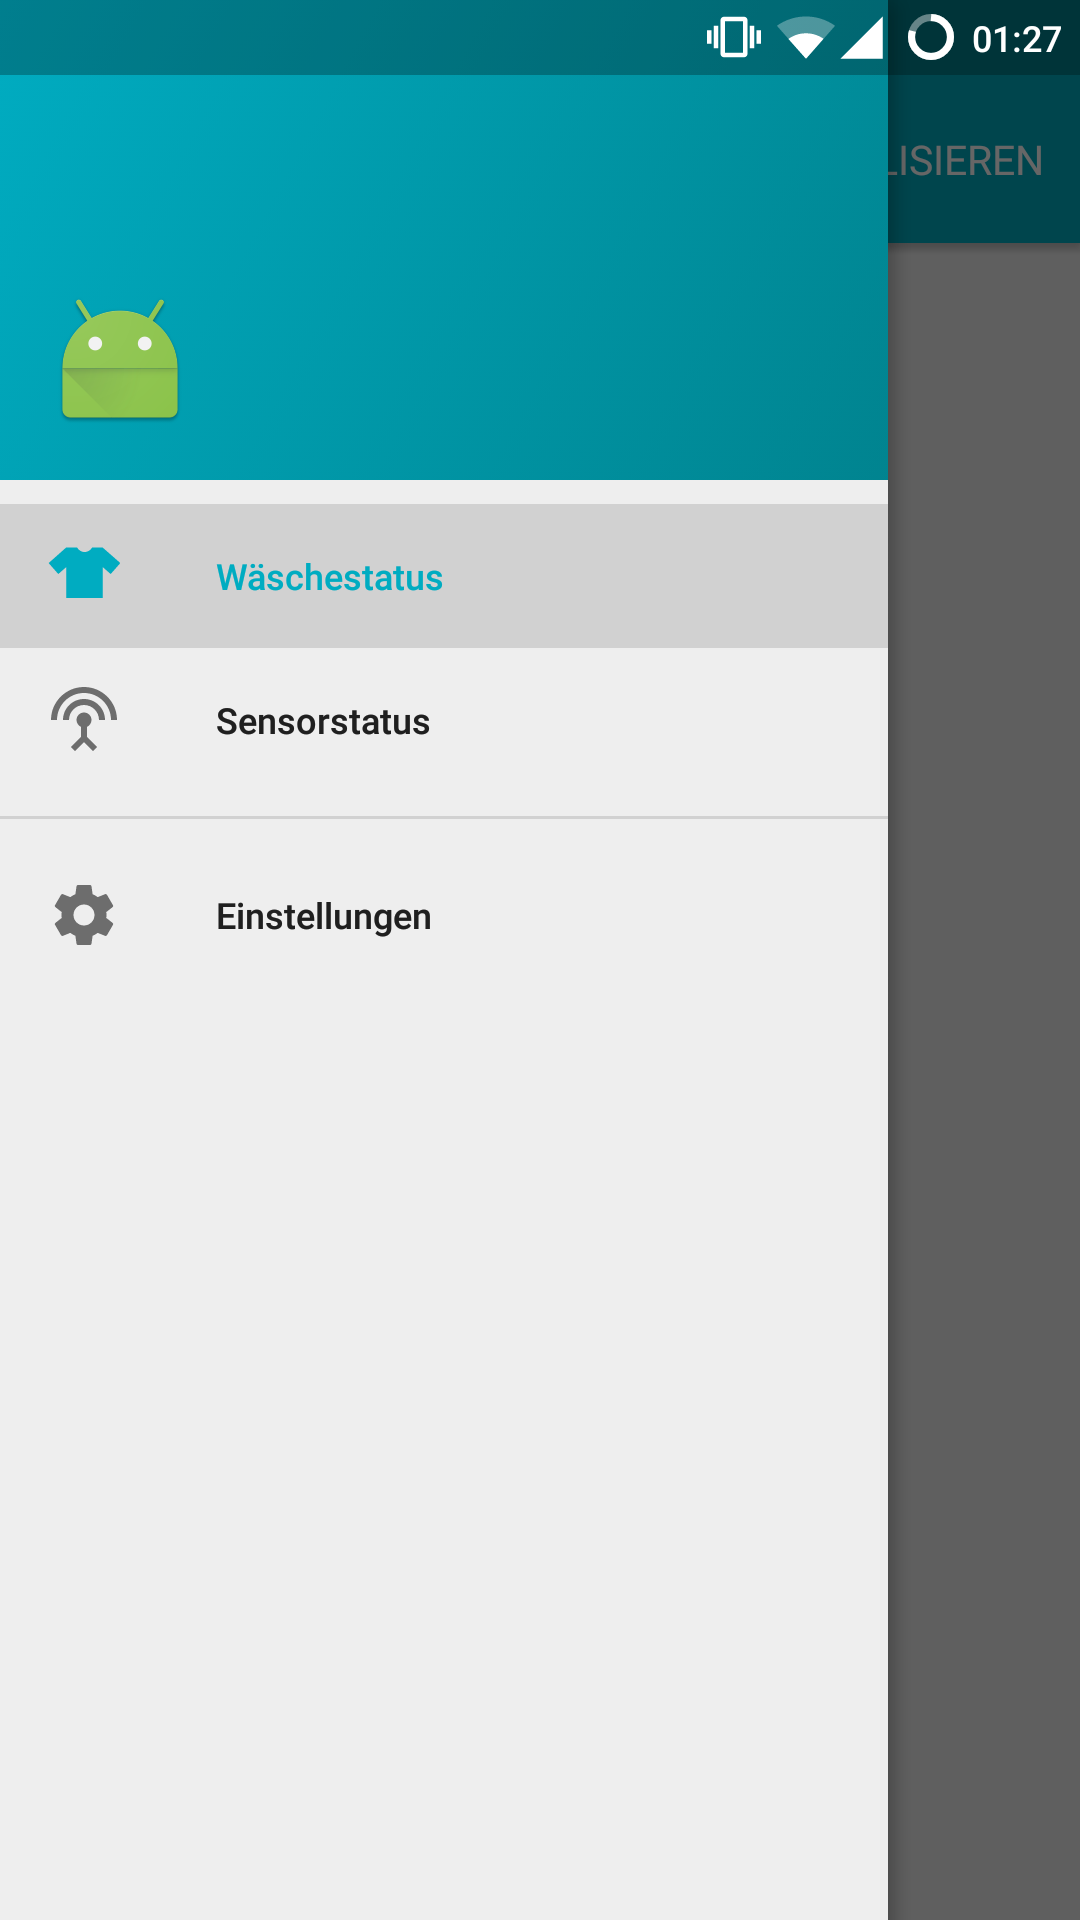
\includegraphics[width=0.5\textwidth]{nav_drawer.png}}
	\caption{Android App nach Sprint 1: Navigationsleiste}
	\label{screenshot_sprint_1_navigation_drawer}
\end{figure}
\clearpage

\subsection{Sprint 2}
Im zweiten Sprint wollten wir die Benutzerfreundlichkeit erhöhen.
Hierbei hat sich schnell heraus gestellt, dass einige Funktionalitäten mit der Hardware des Sensors nicht realisierbar sind. Die Platine lässt in ihrer jetzigen Bauart nicht zu, dass man den Ladezustand der Batterie messen kann. Die Kernpunkte "Wäsche Trocken" und "Vorhersage" haben wir somit bereits im 2. Sprint begonnen. Ein großes Thema war der Betrieb mehrerer Sensoren.
\begin{figure}[htb] 
	\centerline{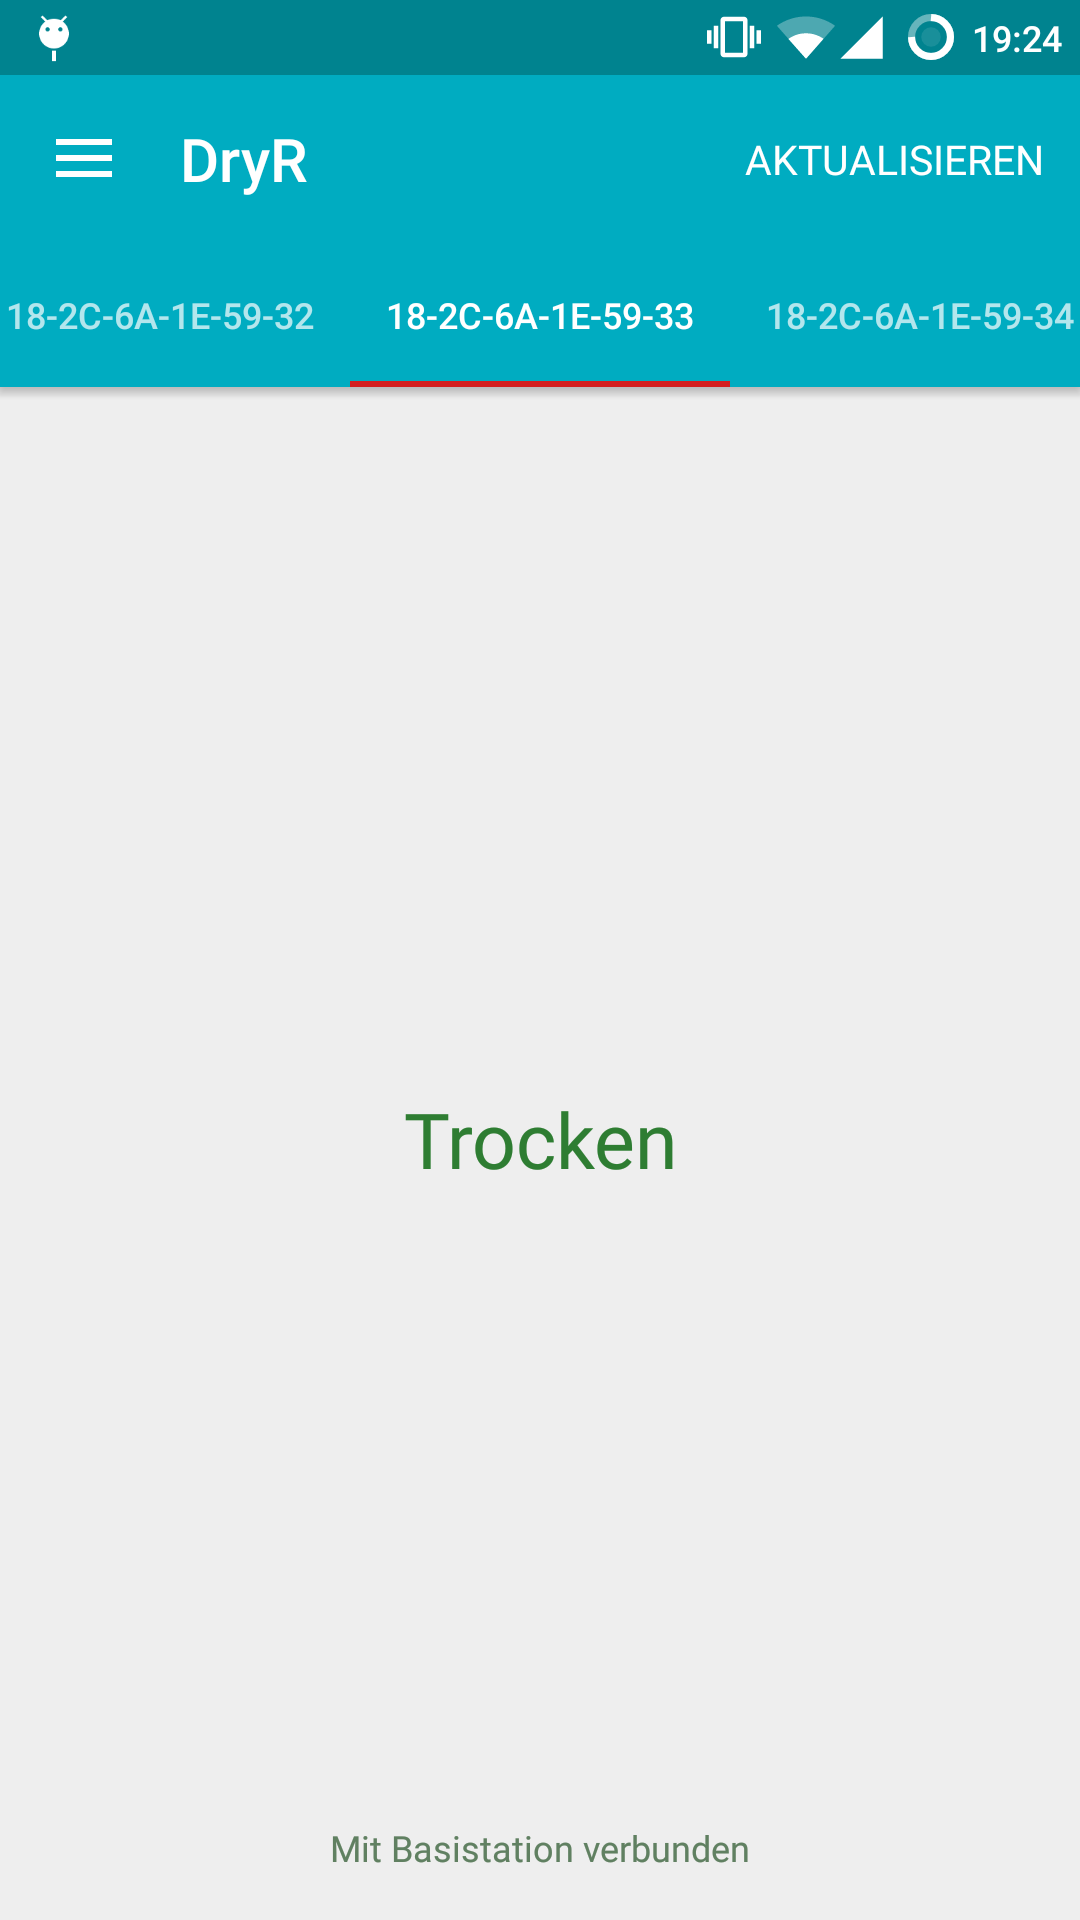
\includegraphics[width=0.5\textwidth]{laundry_status_multiple_sensors.png}}
	\caption{Android App nach Sprint 2: Unterstützung für mehrere Sensoren in Tabs}
	\label{screenshot_sprint_2_laundry_status}
\end{figure}
\begin{figure}[htb] 
	\centerline{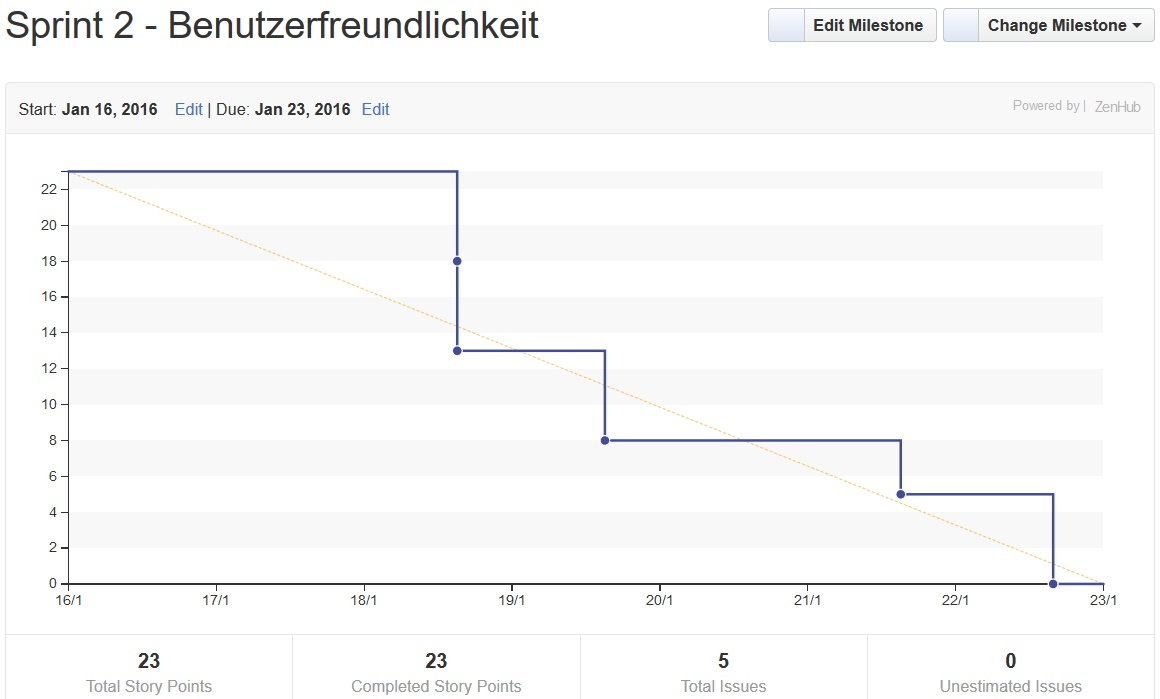
\includegraphics[width=0.7\textwidth]{burndown_sprint2.jpg}}
	\caption{Burndown chart des zweiten Sprints}
	\label{screenshot_sprint_2_burndown}
\end{figure}
\clearpage

\subsection{Sprint 3}
Der dritte Sprint war ursprünglich weiteren Features vorbehalten die nicht unter Grundfunktionalität oder Benutzerfreundlichkeit fallen.
Jedoch hatten wir durch den Emulator und durch den Betrieb mehrerer Sensorgeräte einige Probleme wodurch wir einige Features nicht realisiert haben und uns lieber auf Bugsuche begeben haben. Zudem kann nun die Verbindungsstärke zu den Sensoren in der App angezeigt werden und es wurde ein Diagramm zur Feuchtigkeit der Wäsche erstellt. Weiterhin wurde die Vorhersage weiterentwickelt.
\begin{figure}[htb] 
	\centerline{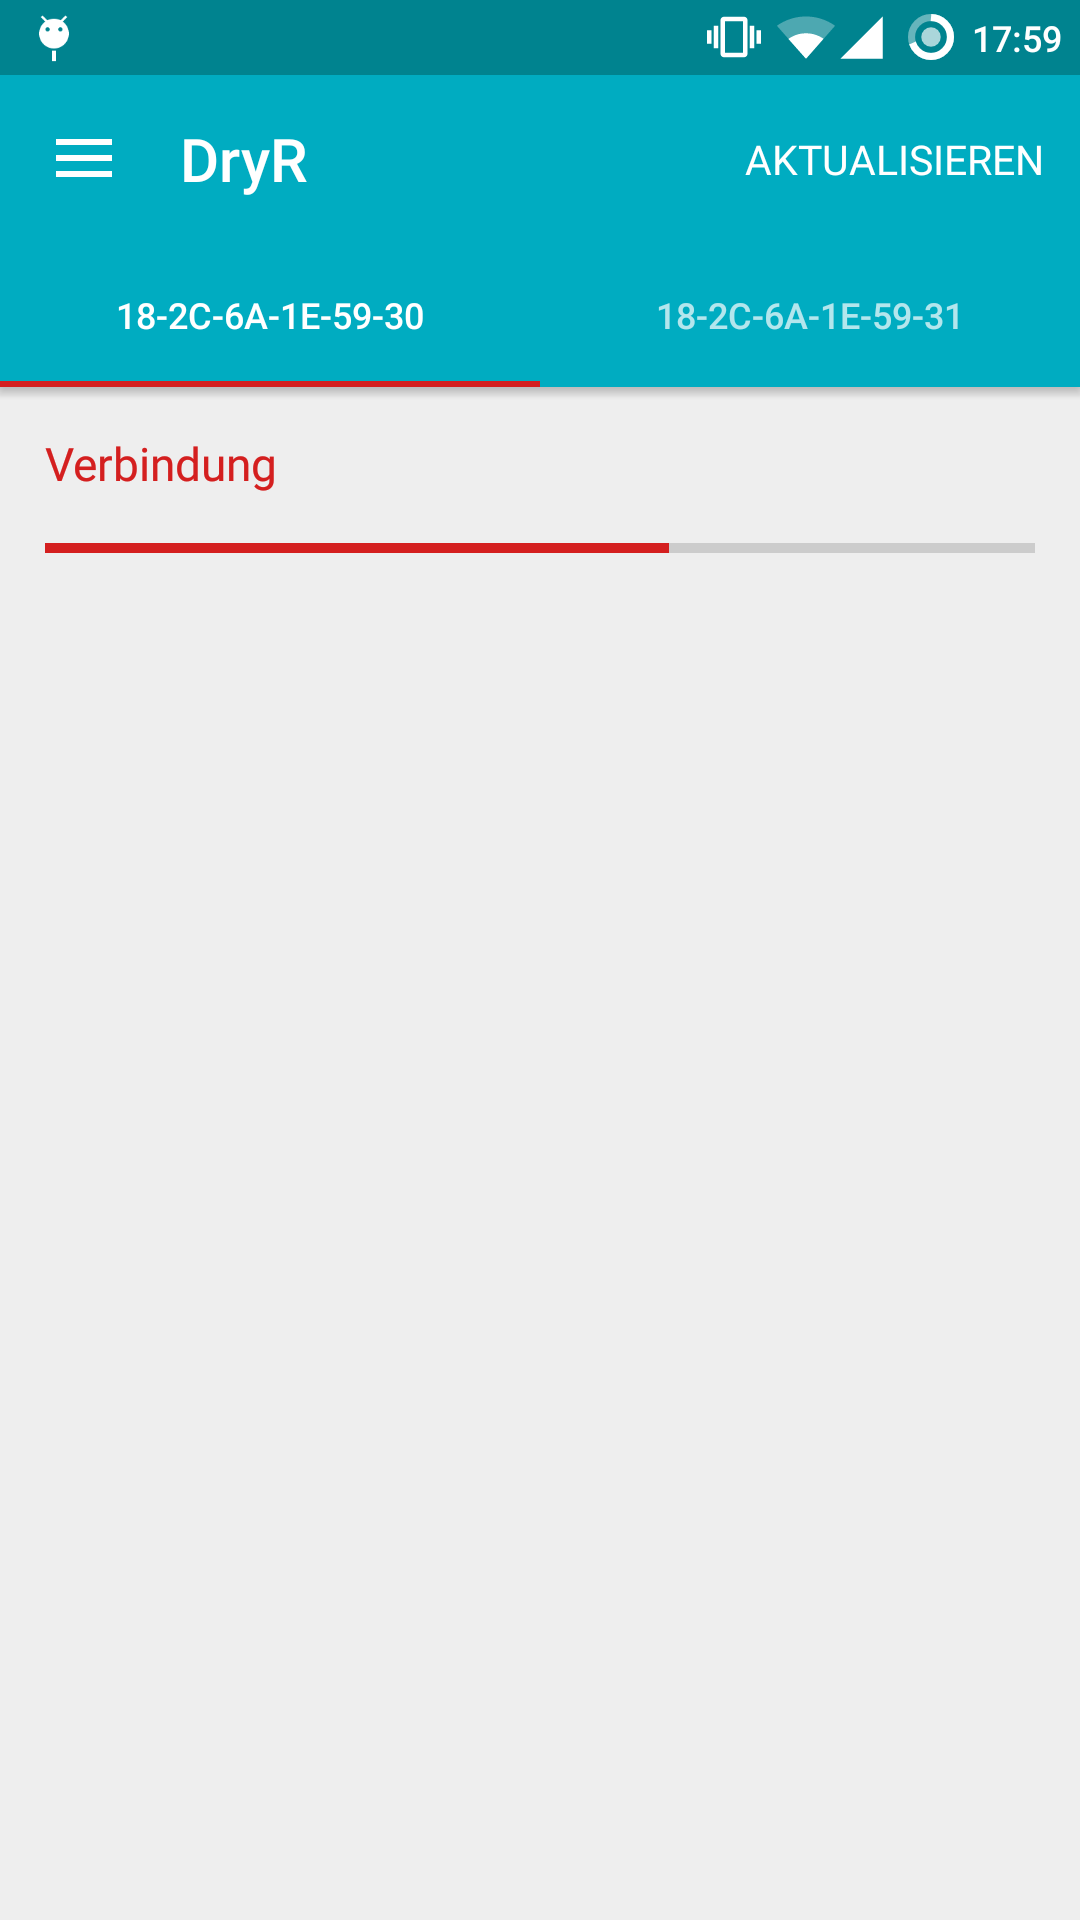
\includegraphics[width=0.5\textwidth]{sensor_status_reception.png}}
	\caption{Android App nach Sprint 3: Unterstützung zur Anzeige der Empfangsstärke der Sensoren in der App}
	\label{screenshot_sprint_3_sensor_status}
\end{figure}
\begin{figure}[htb] 
	\centerline{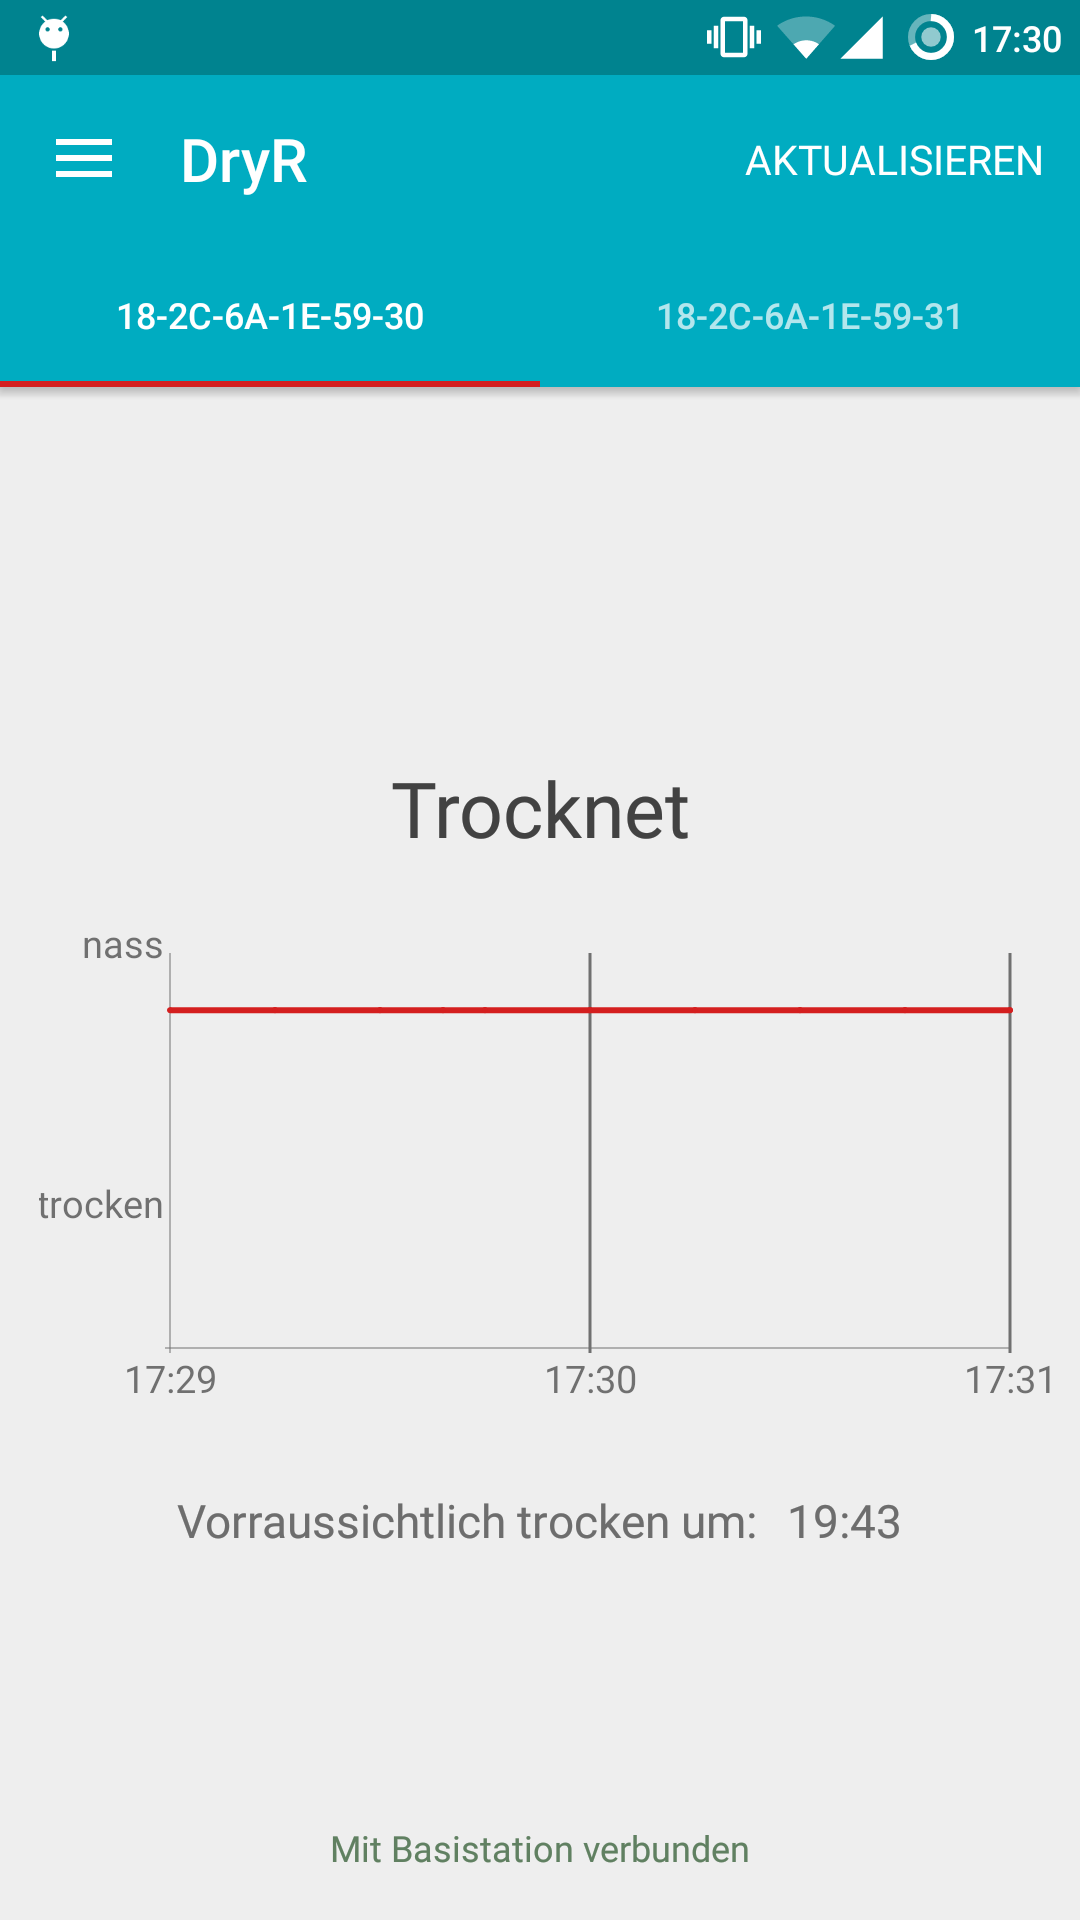
\includegraphics[width=0.5\textwidth]{laundry_status_diagram_forecast.png}}
	\caption{Android App nach Sprint 3: Feuchtigkeitsdiagramm und Vorhersage}
	\label{screenshot_sprint_3_laundry_status}
\end{figure}
\begin{figure}[htb] 
	\centerline{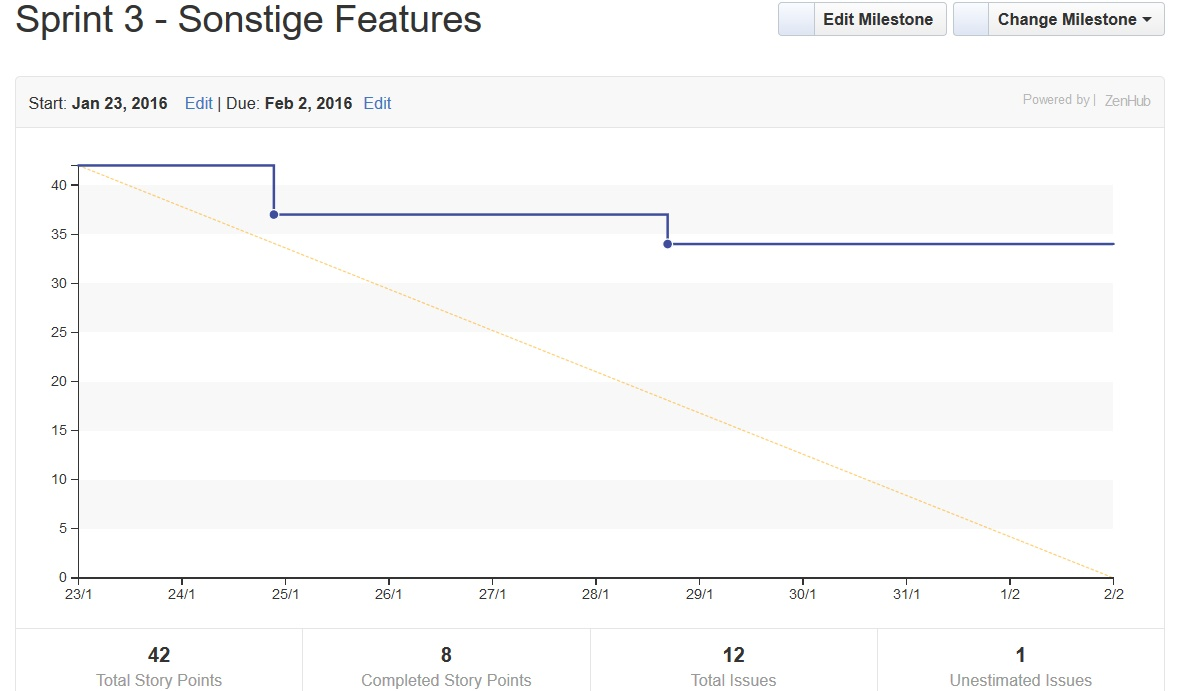
\includegraphics[width=0.7\textwidth]{burndown_sprint3.jpg}}
	\caption{Burndown chart des dritten Sprints, wenig Features umgesetzt, dafür Fehlerbehebungen}
	\label{screenshot_sprint_3_burndown}
\end{figure}
\begin{figure}[htb] 
	\centerline{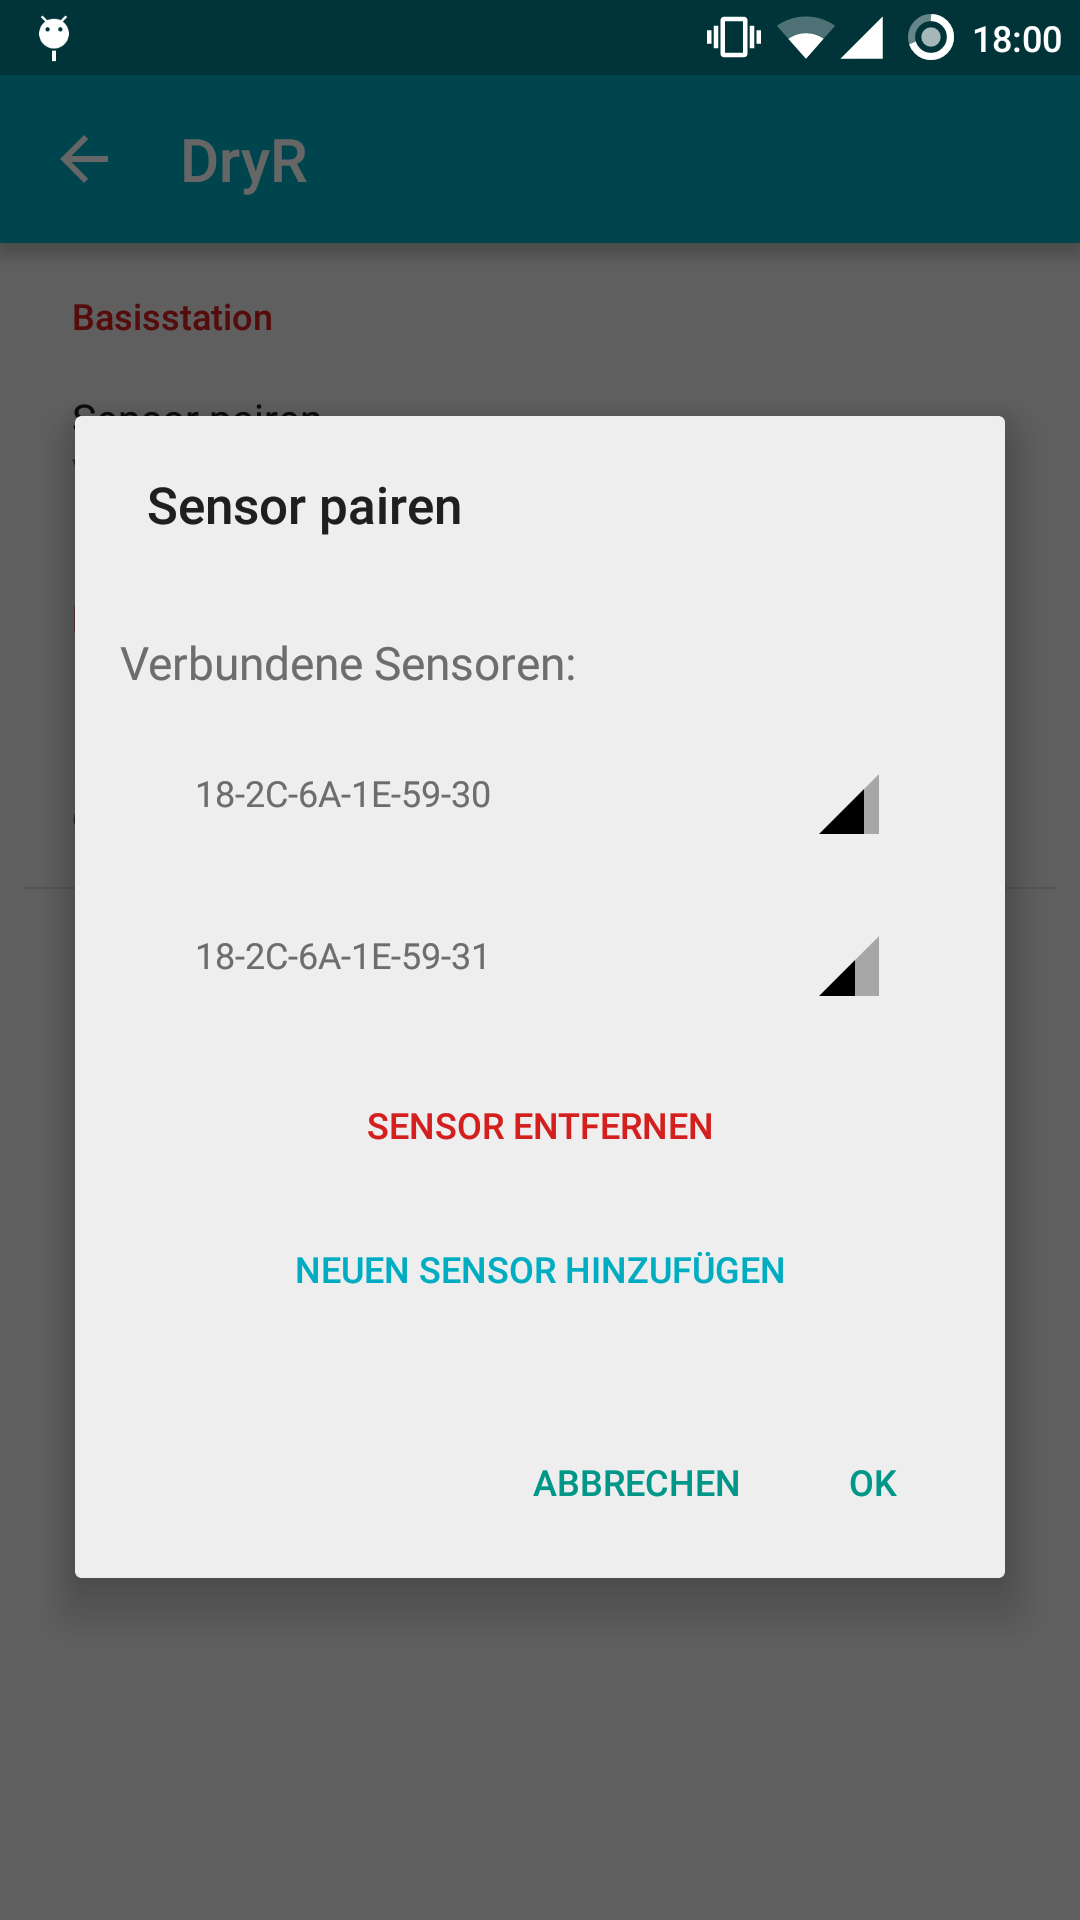
\includegraphics[width=0.5\textwidth]{pair_sensor_dialog_reception.png}}
	\caption{Android App nach Sprint 3: Unterstützung zur Anzeige der Empfangsstärke der Sensoren in der App. Hier: Im Dialog zum Verbinden von Sensoren}
	\label{screenshot_sprint_3_pair_sensor}
\end{figure}
\clearpage
\subsection{Features}
Zu den realisierten Features zählen:
\begin{itemize}
	\item Betrieb mehrerer Geräte: Man kann mehrere Klammern mit einer Basisstation auslesen und die App stellt die Klammern dar.
	\item Verbindungsstärke: zeigt an, wie stark die Verbindung zwischen Sensoren und Basisstation ist.
	\item die Vorhersage: in der man eine geschätzte Uhrzeit gesagt bekommt, zu der die Wäsche trocken ist.
	\item Benachrichtigung: entweder direkt über Einsicht in die App oder Push.
\end{itemize}
Weggefallen sind bzw. nicht realisiert wurden:
\begin{itemize}
	\item Benachrichtigung: über Twitter, LED (am Sensor) oder Email. Lässt sich vielleicht noch bei einem marktreifen Produkt realisieren. 
	\item Regenerkennung: Wir gingen beim Prototypen erstmal nur vom Betrieb in geschlossenen Räumen aus. 
	\item Ladezustand: Hardware der Sensorplatine war für eine Messung nicht ausgelegt
\end{itemize}